\subsection{Siamese Network}

 A method for logically mapping a set of points onto a manifold using a set of previously known matches and non-matches is described by \cite{Hasdell:Siamese}. The goal of this technique is to minimize the distance between matched pairs and maximize the distance between unmatched pairs. This is accomplished using a network architecture know as a \textit{Siamese} network. In this architecture there are two deep neural networks that share weights attached to a final layer that determines the distance between the output of the two hidden networks and minimizes the loss function. To train the network a set of matched and non-matched pairs of inputs is sent through the network and the weights are adjusted to maximize or minimize distance accordingly. This is accomplished using the following loss function \[ L(W, Y, \vec{X}_1, \vec{X}_2) = (1 - Y)\frac{1}{2}(D_W)^2 + (Y)\frac{1}{2}\{max(0, m - (D_W))\}^2\] Where \(D_W\) is the euclidean distance between the two outputs, \textit{m} is a radius beyond which we ignore dissimilar points, and Y is the dissimilar label.

By mapping the inputs onto meaningful locations on a manifold, this method clusters similar inputs close to each other. Using this property we can use the distance layer to decide if two inputs are matched. We simply set a limit for euclidean distance and match if the outputs of the hidden layers are within that limit, as in Figure \ref{siamese}. This lets us use this method for our problem of matching, we treat items as similar to each other if they are aliases for the same entity and different otherwise. To begin with we created the non-matched pairs by choosing other entities with at least one word in common, to avoid the network learning a useless function. This successfully brought the matches close together in the input but failed to properly distance pairs that should be different, as shown in Figure \ref{comp_dif_fail}. Since we never fed the network pairs that were completely different it did not learn to distinguish them from matches. To combat this we created two types of different pairs: ones that share at least one word in common and ones that are completely different.

\begin{figure}
\centering
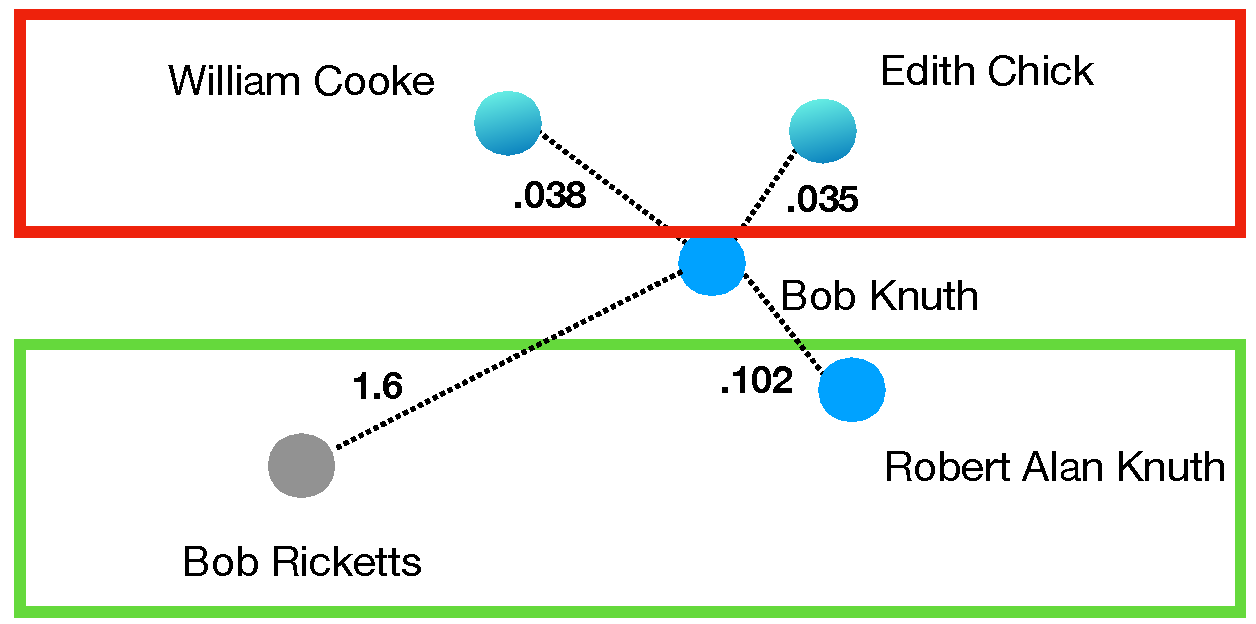
\includegraphics[width=1\linewidth]{word_in_common}
\caption{The model preformed well on somewhat similar names and badly on completely different names}
\label{comp_dif_fail}
\end{figure}
\begin{figure}
\centering
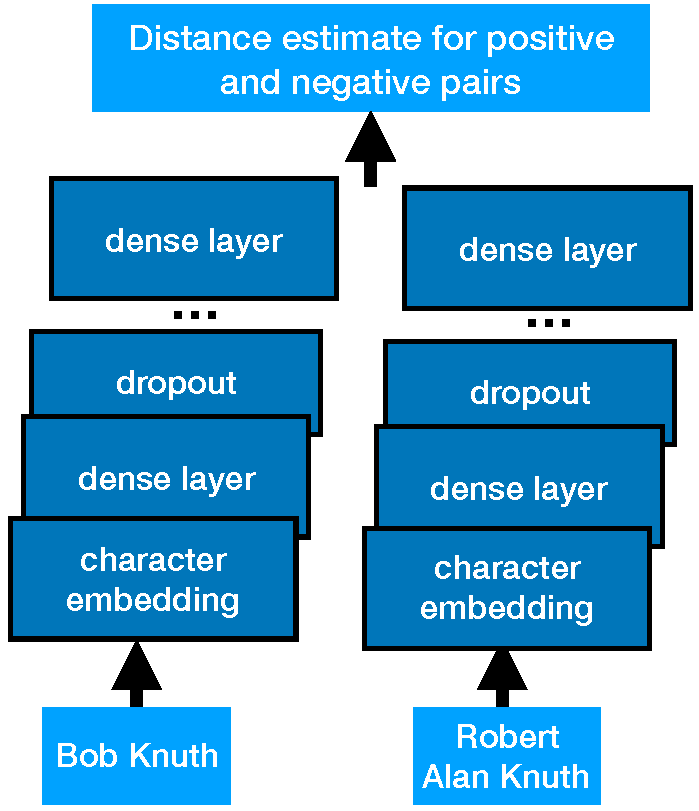
\includegraphics[width=0.5\linewidth]{siamese_arc}
\caption{A siamese network has two networks which share weights which feed into a distance estimator}
\label{siamese}
\end{figure}
